\documentclass[11pt]{article}
\usepackage[latin1]{inputenc}
\usepackage{a4wide}
\usepackage{amsmath}
\usepackage{amsfonts}
\usepackage{amssymb}
\usepackage{graphicx}
\usepackage{enumerate}
\usepackage{epstopdf}
\usepackage{float}
\usepackage{multicol}
\usepackage{hyperref}

\title{Natural Computing, Assignment 1}
\author{Pauline Lauron - sXXXXXXX \and Dennis Verheijden - s4455770 \and Joost Besseling - sXXXXXXX}
\begin{document}
	\maketitle
	
	\section{}
	Due to no eliteness, we can treat the best member as any other member in the pool.
	
	\begin{enumerate}[(a)]
		\item There are 100 individuals, with a mean of 76. That means that the total size of the roulette wheel will be 7600. The current best member has a fitness of 157, so it will occupy $\frac{157}{7600}$th of the roulette wheel. This means that it has roughly a $2\%$ chance of being selected. If we select 100 members, we expect to select the best member $\frac{157}{7600} * 100 \approx 2 $ times.
		
		\item The chance that we don't select the fittest member is $1 - \frac{157}{7600}$. So the chance that we never select it is $\left(1 - \frac{157}{7600}\right)^{100} \approx 0.124$.
	\end{enumerate}

	\section{}
	
	The fitness function is \[ f(x) = x^2. \]
	
	The members of the pool are $x=3, x=5, \text{and} x=7$. So the total fitness is $3^2 + 5^2 + 7^2 = 83$. The chance to select each individual is: 
	\begin{itemize}
		\item[$x=3:$] $9/83 \approx 0.108$,
		
		\item[$x=5:$] $25/83 \approx 0.301$,
		
		\item[$x=5:$] $49/83 \approx 0.590$.
		 
	\end{itemize}

	When using the alternative selection function 
	\[
		f_1(x) = x^2 + 8,
	\] 
	
	the total fitness is $83 + 24 = 107$ and
	we obtain the following results: 
	
		\begin{itemize}
		\item[$x=3:$] $17/107 \approx 0.159$,
		
		\item[$x=5:$] $33/107 \approx 0.308$,
		
		\item[$x=5:$] $57/107 \approx 0.533$.
		
	\end{itemize}

We can see that the second function yields a lower selection pressure. This is because the relative boost of 8 is much higher for the less fit individuals. It almost doubles the fitness of the $x=3$ individual, and only amounts to a $0.16$-th increase in fitness of the $x=7$ individual.

\section{}
\begin{enumerate}[(a)]
\item When running the algorithm with $n=100$ for 1500 iterations, we can observe the result found in figure \ref{fig:mc}. We can see that the Monte-Carlo search as specified in the assignment did not find the optimal solution.

\item Running the algorithm ten times, the algorithm finds the optimal solution 0 times.

\end{enumerate}

\begin{figure}[H]
\centering
\includegraphics[width=0.75\textwidth]{images/monte_carlo.eps}
\caption{Monte Carlo Search for the Counting Ones problem, ran 10 times.}
\label{fig:mc}
\end{figure}

\section{}
\begin{enumerate}[(a)]
\item When running the (1+1)-GA algorithm for the Counting Ones problem, we found the results from figure \ref{fig:ga}.
\item As we can observe from our results, the algorithm found the optimum 10 times out of 10 runs.
\item If we compare these results to those of the Monte-Carlo algorithm, we can easily see that the Genetic Algorithm is a significant improvement, as the Monte-Carlo algorithm did not find the optimum once and the GA algorithm every time.
\end{enumerate}

\begin{figure}[H]
\centering
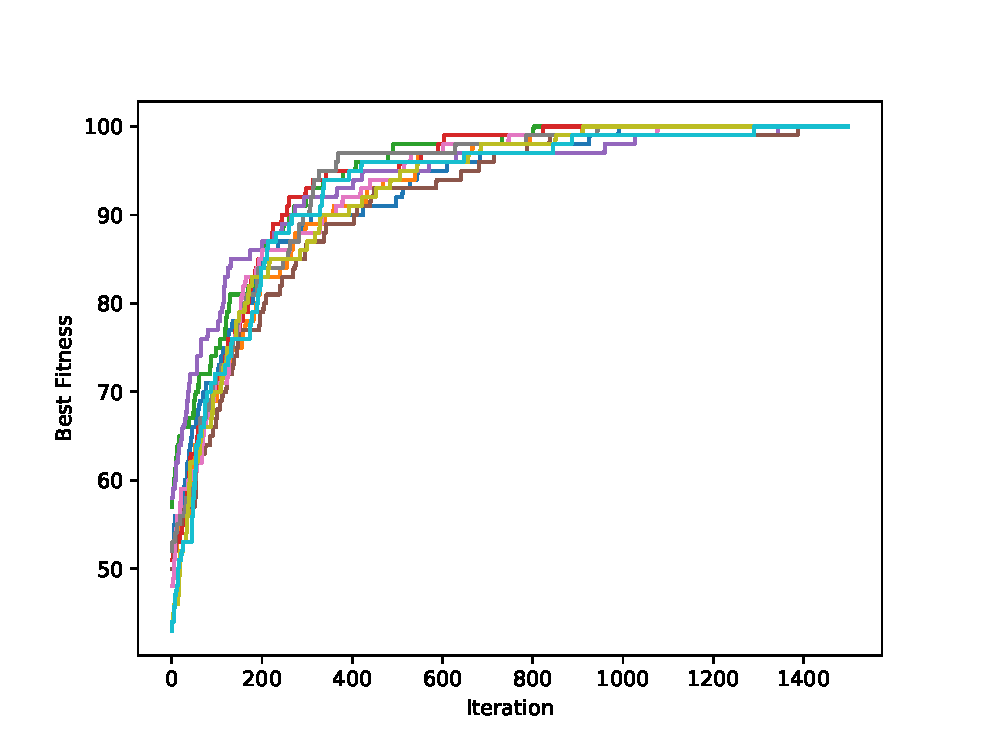
\includegraphics[width=0.75\textwidth]{images/ga.eps}
\caption{(1+1)-GA for the Counting Ones problem, ran 10 times.}
\label{fig:ga}
\end{figure}

\section{}
Suitable fonction : $F = \{\wedge,\rightarrow, \vee,\leftrightarrow \}$
\newline Terminal set : $T = \{x,y,z,true\}$
\newline S-expression : $ (\rightarrow (\land\ x\ true)(\lor (\lor\ x\ y)(\leftrightarrow z(\land\ x\ y))) $

\section{}
For this exercise we had to make some changes to the primitive function set, since \textit{log} must be greater than zero, \textit{exp} could not have a too large argument (because of overflows) and \textit{div} since its second argument cannot be zero. For this we created protected functions.

For the implementation of this assignment we used the python module \texttt{DEAP}. For the tree structure we used a \texttt{genHalfAndHalf} tree, since we think it has more flexibility than using a \textit{grown} or \textit{full} tree. 

In figure \ref{fig:best_fitness}, we see the best of generation fitness per generation. What we can observe from this figure and the output of the algorithm is that the best solution has a \textit{-sum of absolute errors} of $-0.02$, which is pretty good. It is not perfect, however we doubt that it can be perfect. Since the algorithm could not find a solution within 1000 generations, although it kept (marginally) improving. This could be due to rounding errors in the given output, or that these numbers are not actually generated by a function that can be made using the functions in our primitive set. Another solution may be to allow mutations. We did a preliminary test, which converged on an error of $-0.0008$, so this could be possible.

In figure \ref{fig:best_size}, we see the best of generation size per generation. From this figure, we may observe that the best solution of the algorithm does not necessarily have to grow in size to improve.

After repeating this experiment for 100 epochs, we believe to have found the solution. The algorithm managed to find an individual whose error was $-8.68353e-16$, which is near $0$. The results may be found in figure \ref{fig:best_fitness2}-\ref{fig:best_size2}. The latter may be more evidence to the hypothesis about the best of generation size. The function that achieved this error is the following:

\begin{verbatim}
add(mul(add(x, mul(add(mul(x, x), x), x)), x), x)
\end{verbatim}

\begin{multicols}{2}
\centering
\begin{figure}[H]
\includegraphics[width=0.45\textwidth]{images/genetic_best_fitness.eps}
\caption{Best of generation fitness per generation.}
\label{fig:best_fitness}
\end{figure}
\begin{figure}[H]
\includegraphics[width=0.45\textwidth]{images/genetic_best_size.eps}
\caption{Best of generation size per generation.}
\label{fig:best_size}
\end{figure}
\end{multicols}

\begin{multicols}{2}
\centering
\begin{figure}[H]
\includegraphics[width=0.45\textwidth]{images/genetic_best_fitness2.eps}
\caption{Best of generation fitness per generation.}
\label{fig:best_fitness2}
\end{figure}
\begin{figure}[H]
\includegraphics[width=0.45\textwidth]{images/genetic_best_size2.eps}
\caption{Best of generation size per generation.}
\label{fig:best_size2}
\end{figure}
\end{multicols}


\end{document}